\documentclass[12pt]{article}
\usepackage{fontspec}
\usepackage{polyglossia}
\setmonofont{Courier New}
\setmainlanguage{farsi}
\setotherlanguage{english}
\newfontfamily\persianfont[Script=Arabic]{XBZar}
\usepackage{graphicx}
\usepackage{geometry}
\usepackage{hyperref}
\geometry{a4paper, margin=2.5cm}
\usepackage{setspace}
\usepackage{url}
\onehalfspacing
\usepackage{titling}
\usepackage{float}
\usepackage{etoolbox}
\usepackage[backend=biber,style=numeric,sorting=none]{biblatex}
%%%%%%%%%%%%%%%%%%%%%%%%%%%%%%%%%%%%%%%%%%%%%%%%%%%%%%%%%%%%%%%%%%%%%%%%%%%%%
\makeatletter
\newcommand{\persiandigit}[1]{%
	\ifcase#1 ۰\or ۱\or ۲\or ۳\or ۴\or ۵\or ۶\or ۷\or ۸\or ۹\fi
}
\DeclareFieldFormat{labelnumber}{\persiandigit{#1}}
\makeatother
%%%%%%%%%%%%%%%%%%%%%%%%%%%%%%%%%
\newcommand{\persianordinal}[1]{%
	\ifcase#1
	\or اول%
	\or دوم%
	\or سوم%
	\or چهارم%
	\or پنجم%
	\or ششم%
	\or هفتم%
	\or هشتم%
	\or نهم%
	\or دهم%
	\or یازدهم%
	\or دوازدهم%
	\or سیزدهم%
	\or چهاردهم%
	\or پانزدهم%
	\or شانزدهم%
	\or هفدهم%
	\or هجدهم%
	\or نوزدهم%
	\or بیستم%
	\else #1\fi
}

\newcommand{\persianordinalpage}{\persianfont\persianordinal{\value{page}}}


%%%%%%%%%%%%%%%%%%%%%%%%%%%%%%%%%%%%%%%%%%%%%%%%%%%%%%%%%%%%%%%%%%%%%%%%%%%%%
\begin{filecontents}{\jobname.bib}
	@online{a1,
		url = {https://www.geeksforgeeks.org/c/c-program-demonstrate-fork-and-pipe/}
	}
\end{filecontents}

\addbibresource{\jobname.bib}

\defbibheading{bibliography}[]{%
	\begin{RTL}
		\section*{مراجع}
	\end{RTL}
}

%%%%%%%%%%%%%%%%%%%%%%%%%%%%%%%%%%%%%%%%%%%%%%%%%%%%%%%%%%%%%%%%%%%%%%%%%%%%%

\begin{document}
	
	% ==============================
	% Title Page
	% ==============================
	\begin{titlepage}
		\centering
		\vspace*{1cm}
		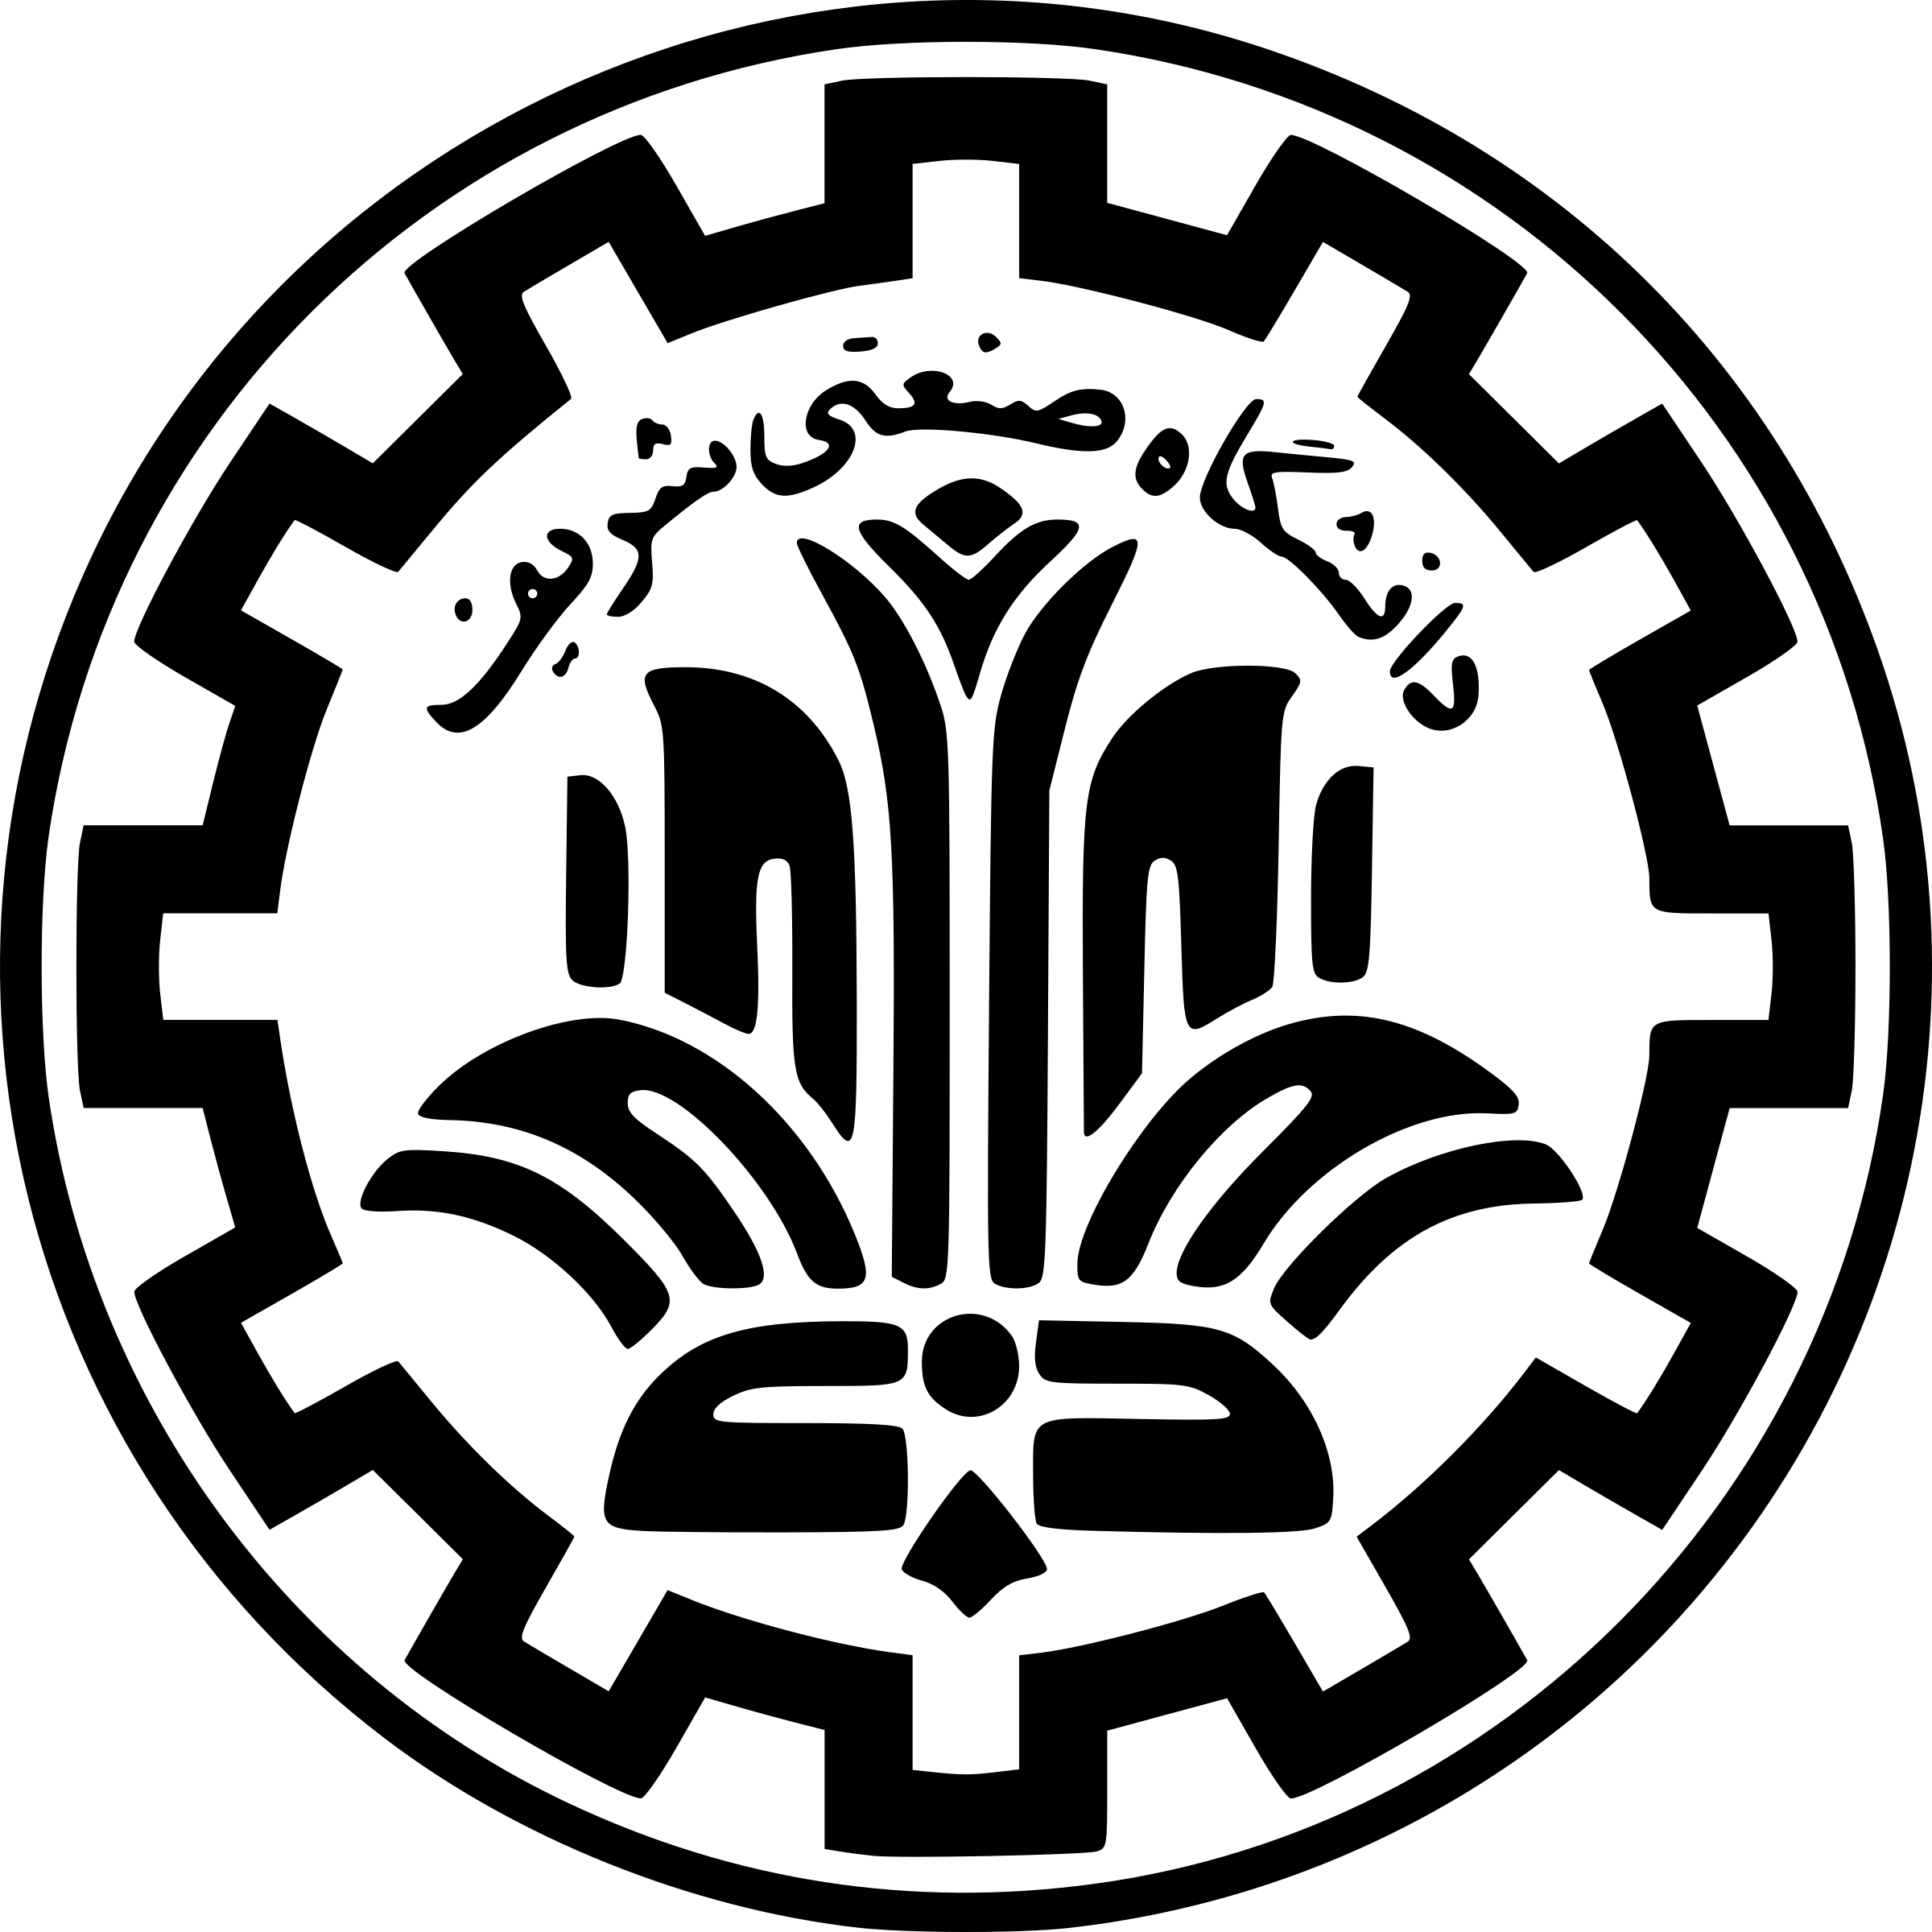
\includegraphics[width=4cm]{sharif.png}\\[1.5cm]
		{\Large\textbf{دانشگاه صنعتی شریف}}\\[0.5cm]
		{\large\textbf{دانشکده‌ٔ مهندسی کامپیوتر}}\\[1.5cm]
		{\Huge\textbf{گزارش کار آزمایشگاه}}\\[0.5cm]
		{\LARGE\textbf{آزمایشگاه سیستم‌های عامل}}\\[2cm]
		
		\textbf{گزارش آزمایش شماره ۷}\\
		(آشنایی با ریسه‌ها)
		
		\vfill
		\begin{tabular}{rl}
			\textbf{شماره‌ی گروه:} & ۲۰ \\
			\textbf{گروه:} &
			ارشیا یوسف‌نیا (۴۰۱۱۱۰۴۱۵) \\
			& محمدعارف زارع زاده (۴۰۱۱۰۶۰۱۷) \\
			\textbf{استاد درس:} & دکتر بیگی \\
			\textbf{تاریخ:} & تابستان ۱۴۰۴ \\
		\end{tabular}
	\end{titlepage}
	
	% ==============================
	% Persian Ordinal Page Numbering
	% ==============================
	\clearpage
	\setcounter{page}{1}
	\renewcommand{\thepage}{\persianordinalpage}
	
	\tableofcontents
	\clearpage
	\listoffigures
	%\clearpage
	%\listoftables
	
	% ==============================
	% Switch to Persian Digits (۱, ۲, ۳, ...)
	% ==============================
	\clearpage
	\setcounter{page}{1}
	\pagenumbering{arabic}
	\renewcommand{\thepage}{\persianfont\arabic{page}}
	
	
	% ==============================
	% Main Content
	% ==============================
	\section{آشنایی اولیه}
	\subsection{}
	وارد سیستم لینوکس می‌شویم.
	\subsection{}
	در ادامه با کد شکل \ref{img:1} یک ریسه میسازیم که صرفا داخل خود یک پیام چاپ میکند. داخل ریسهٔ اصلی با توقف برای یک زمان، زمانی ریسهٔ اصلی را خاتمه میدهیم که ریسهٔ دوم هم تمام شده باشد. این روش تضمینی نیست ولی برای این حالت ساده کار می‌کند. شکل \ref{img:2} گام‌های کامپایل و اجرا و را نشان می‌دهد.
	\begin{figure}[H]
		\centering
		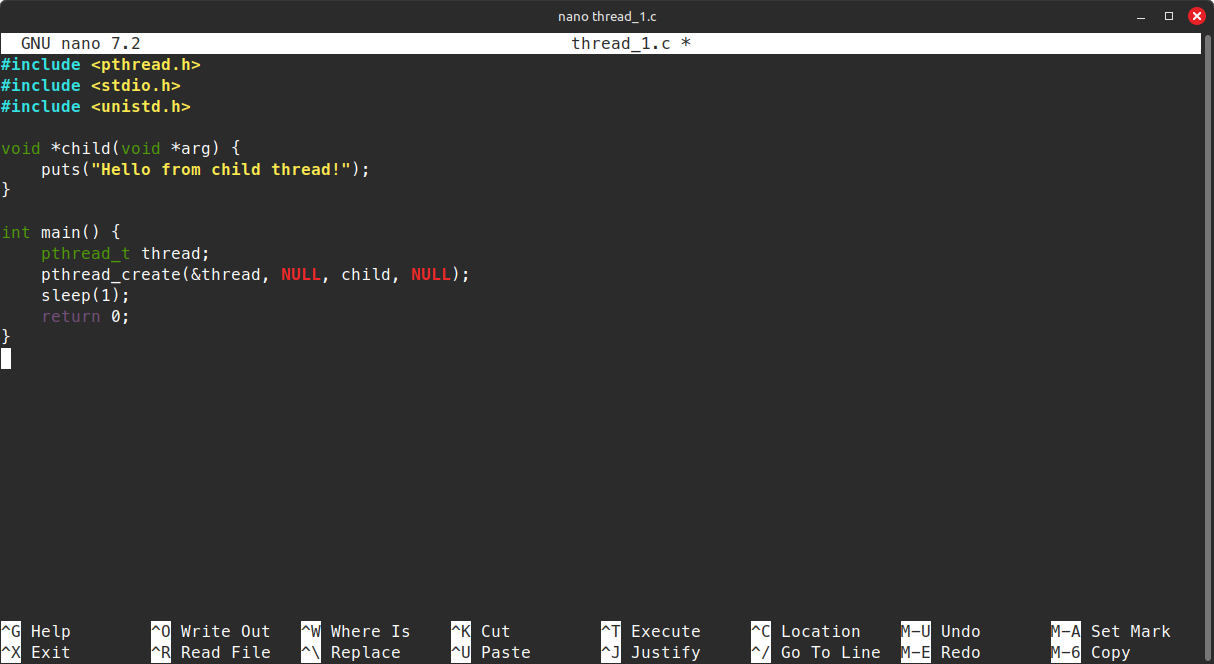
\includegraphics[width=\textwidth]{report7-resources/1.png}
		\caption{ایجاد یک ریسهٔ جدید و چاپ یک پیام در آن}
		\label{img:1}
	\end{figure}
	\begin{figure}[H]
		\centering
		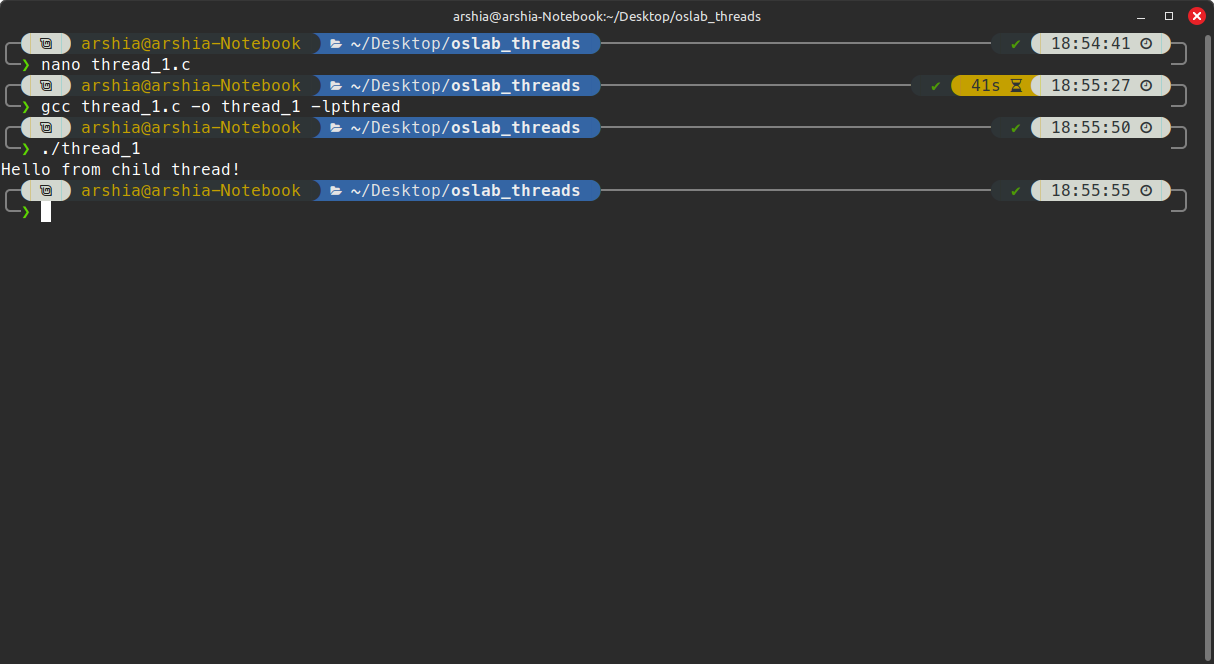
\includegraphics[width=\textwidth]{report7-resources/2.png}
		\caption{گام‌های کامپایل و اجرای برنامه شکل \ref{img:1}}
		\label{img:2}
	\end{figure}
	\subsection{}
	در این قسمت با \textenglish{pthread\_create} و \textenglish{pthread\_join} یک برنامه می‌نویسیم که یک ریسهٔ جدید درست کند و هم در آن و هم در ریسهٔ اصلی شمارهٔ پردازه را چاپ کند. این اعداد باید یکسان باشند. شکل \ref{img:3} این برنامه را نشان می‌دهد و شکل \ref{img:4} مراحل کامپایل و اجرای آن را نشان می‌دهد.
	\begin{figure}[H]
		\centering
		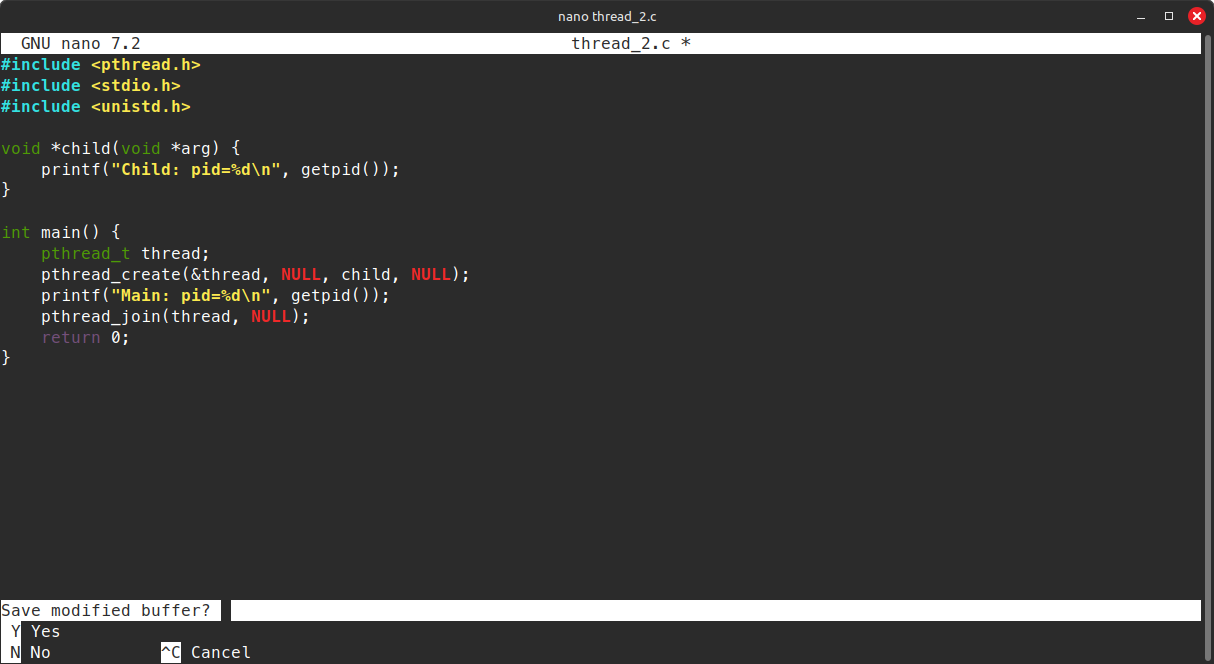
\includegraphics[width=\textwidth]{report7-resources/3.png}
		\caption{چاپ شمارهٔ پردازه در ریسهٔ اصلی و ریسهٔ جدید}
		\label{img:3}
	\end{figure}
	\begin{figure}[H]
		\centering
		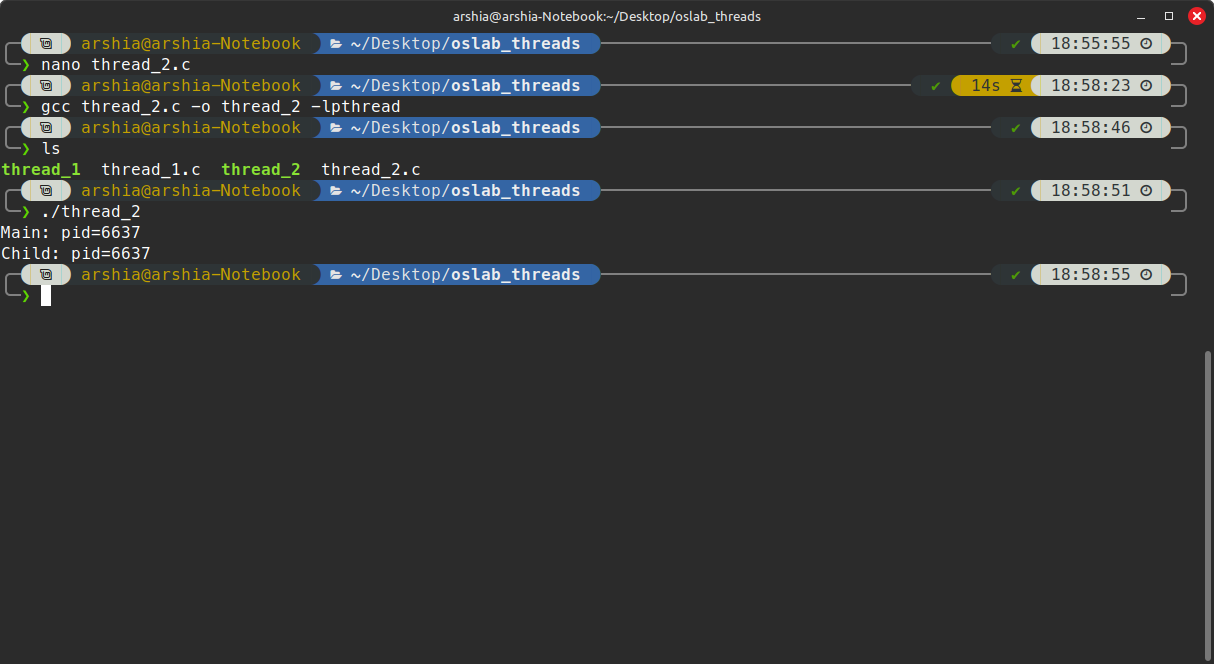
\includegraphics[width=\textwidth]{report7-resources/4.png}
		\caption{گام‌های کامپایل و اجرای برنامه شکل \ref{img:3}}
		\label{img:4}
	\end{figure}
	\subsection{}
	در این قسمت یک متغیر عمومی به برنامه اضافه می‌کنیم و در هر دو ریسهٔ برنامه قبل مقدار آن را تغییر می‌دهیم و بررسی می‌کنیم. این آزمایش مشترک بودن حافظهٔ ریسه‌ها را نشان می‌دهد. در شکل \ref{img:5} متن برنامه و در شکل \ref{img:6} هم کامپایل و اجرای آن آمده است.
	\begin{figure}[H]
		\centering
		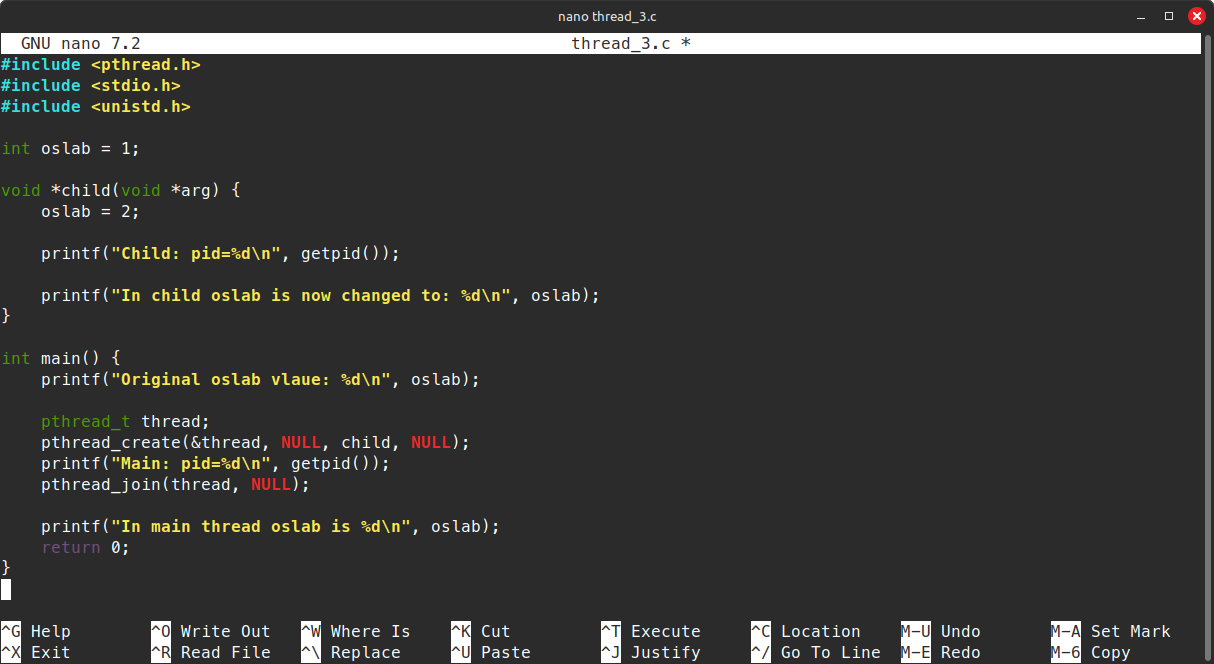
\includegraphics[width=\textwidth]{report7-resources/5.png}
		\caption{دسترسی به متغیر عمومی از دو ریسهٔ متفاوت}
		\label{img:5}
	\end{figure}
	\begin{figure}[H]
		\centering
		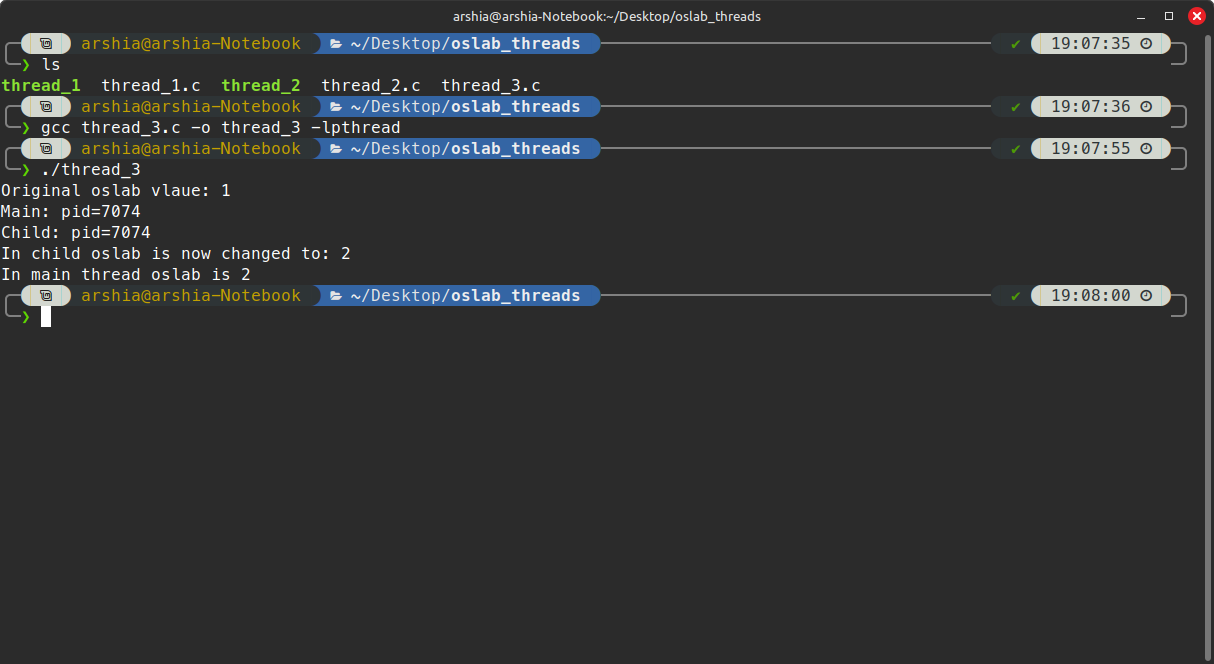
\includegraphics[width=\textwidth]{report7-resources/6.png}
		\caption{گام‌های کامپایل و اجرای برنامه شکل \ref{img:5}}
		\label{img:6}
	\end{figure}
	
	\subsection{}
	اکنون یک برنامه می‌نویسیم که یک ریسهٔ جدید درست کند که در آن عددی که ورودی گرفته‌ایم داده می‌شود و برنامه از عدد ۲ تا آن عدد را جمع می‌کند و حاصل را نمایش می‌دهد. شکل \ref{img:7} این برنامه را نشان می‌دهد و شکل \ref{img:8} کامپایل و اجرای آن را نشان می‌دهد.
	
	\begin{figure}[H]
		\centering
		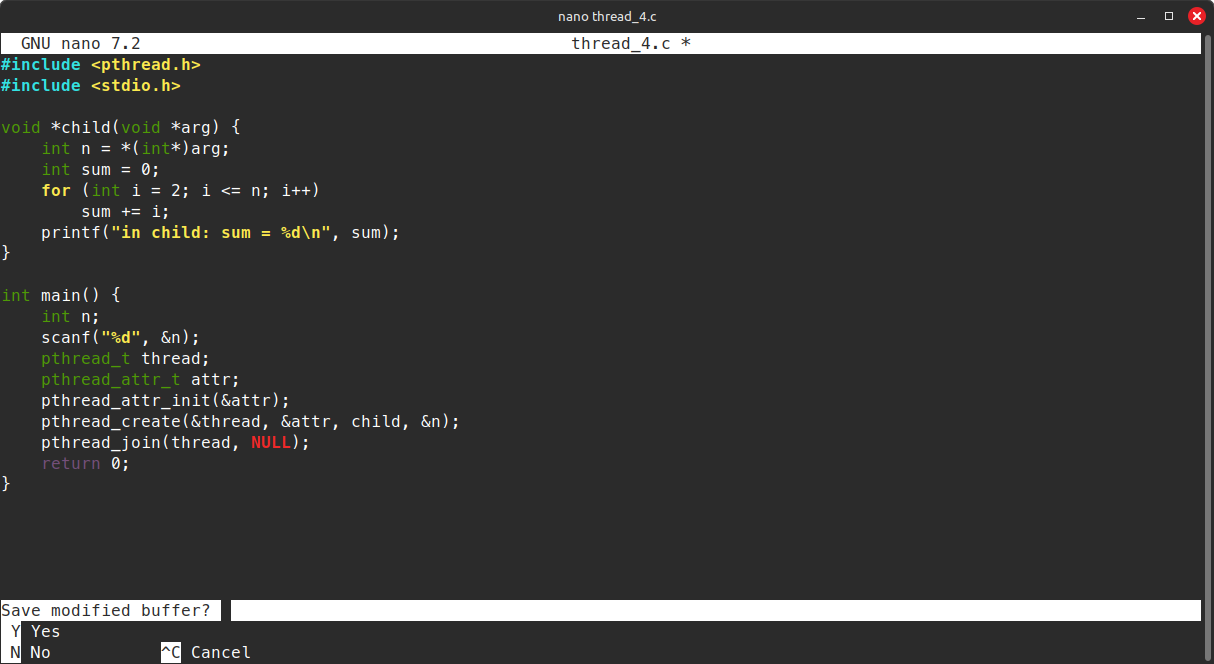
\includegraphics[width=\textwidth]{report7-resources/7.png}
		\caption{اعداد ۲ تا عدد ورودی در ریسهٔ جدید جمع زده می‌شوند}
		\label{img:7}
	\end{figure}
	\begin{figure}[H]
		\centering
		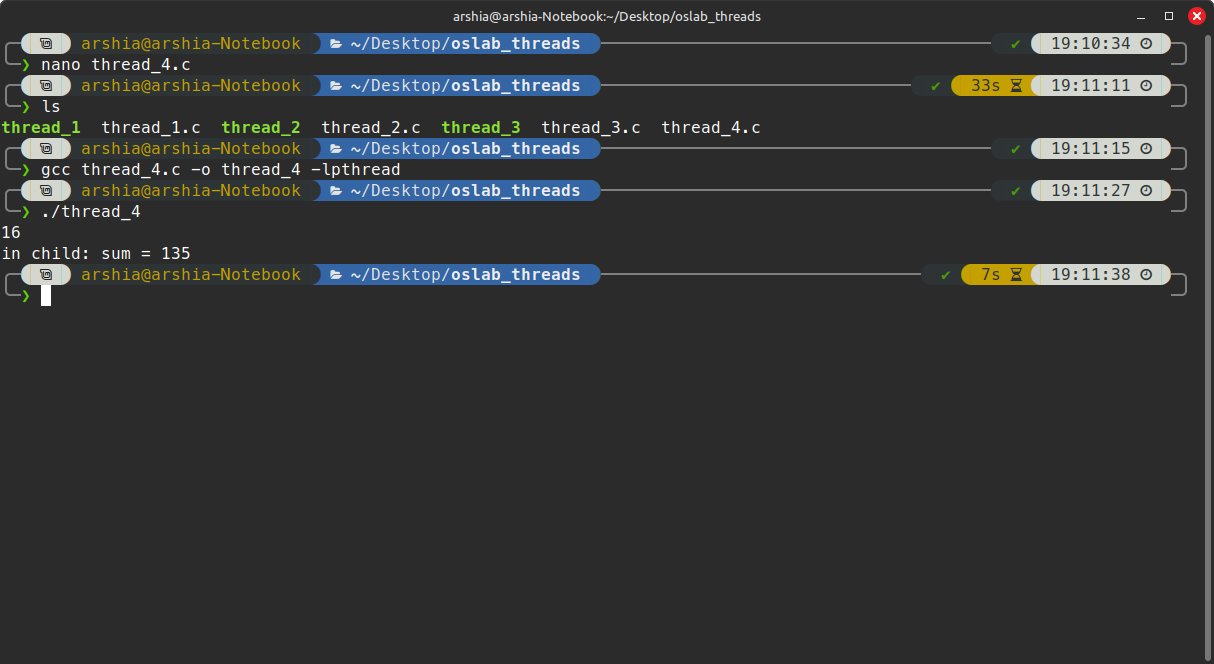
\includegraphics[width=\textwidth]{report7-resources/8.png}
		\caption{گام‌های کامپایل و اجرای برنامه شکل \ref{img:7}}
		\label{img:8}
	\end{figure}
	\newpage
	\section{ریسه‌های چندتایی}
	در این قسمت ۵ ریسه می‌سازیم و در هر کدام یک پیام چاپ می‌کنیم. در نهایت زمانی ریسهٔ اصلی را تمام می‌کنیم که همه ریسه‌ها تمام شده باشند. شکل \ref{img:9} برنامه را نشان می‌دهد. اجرا و خروجی در شکل \ref{img:10} آمده است.
	\begin{figure}[H]
		\centering
		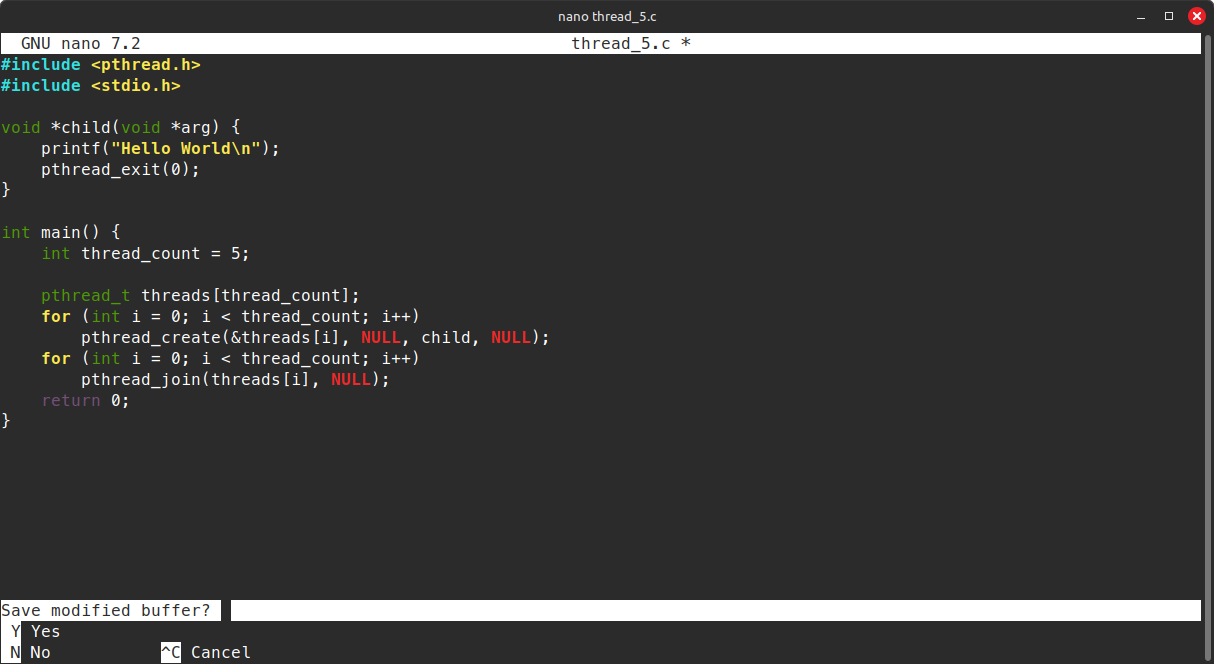
\includegraphics[width=\textwidth]{report7-resources/9.png}
		\caption{ایجاد چند ریسه}
		\label{img:9}
	\end{figure}
	\begin{figure}[H]
		\centering
		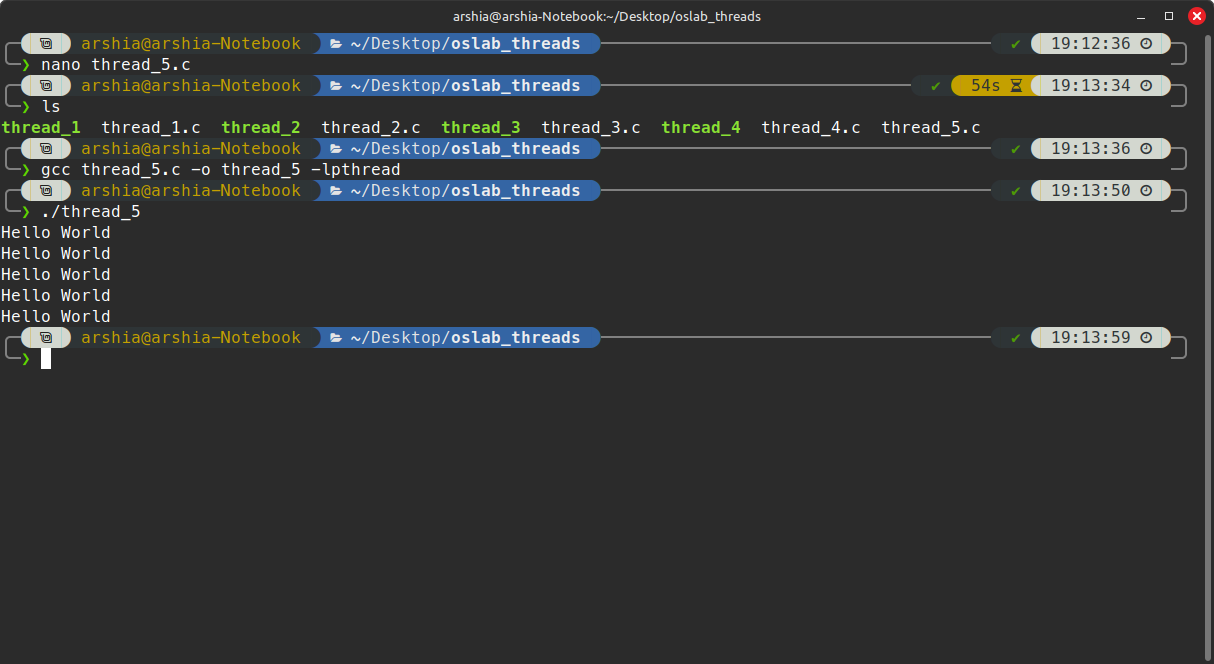
\includegraphics[width=\textwidth]{report7-resources/10.png}
		\caption{گام‌های کامپایل و اجرای برنامه شکل \ref{img:9}}
		\label{img:10}
	\end{figure}
	\newpage
	\section{تفاوت بین پردازه‌ها و ریسه‌ها}
	\subsection{}
	برای سهولت گزارش تابع این قسمت را در کد قسمت بعد آورده‌ایم.
	\subsection{}
	در این قسمت یک متغیر عمومی را در ریسه تغییر می‌دهیم و اثر آن بر ریسهٔ اصلی را میبینیم. شکل \ref{img:11} برنامه را نشان می‌دهد و شکل \ref{img:12} نتیجهٔ آن را نشان می‌دهد.
	\begin{figure}[H]
		\centering
		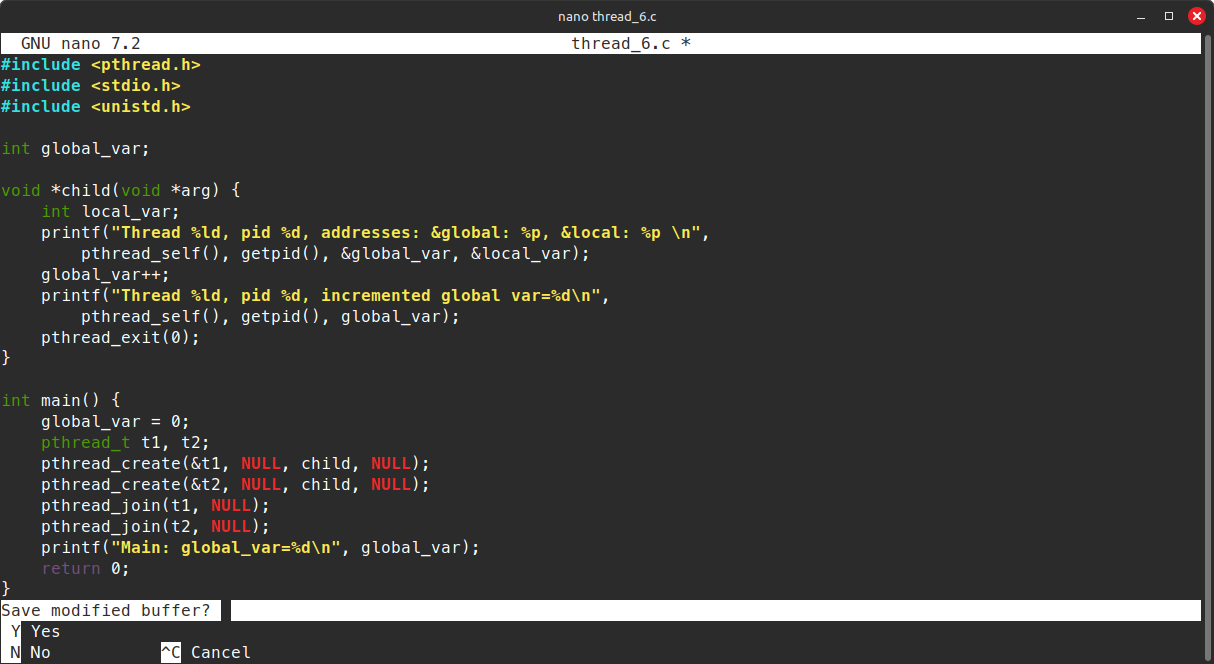
\includegraphics[width=\textwidth]{report7-resources/11.png}
		\caption{دسترسی به متغیر عمومی در ریسهٔ اصلی و فرعی}
		\label{img:11}
	\end{figure}
	\begin{figure}[H]
		\centering
		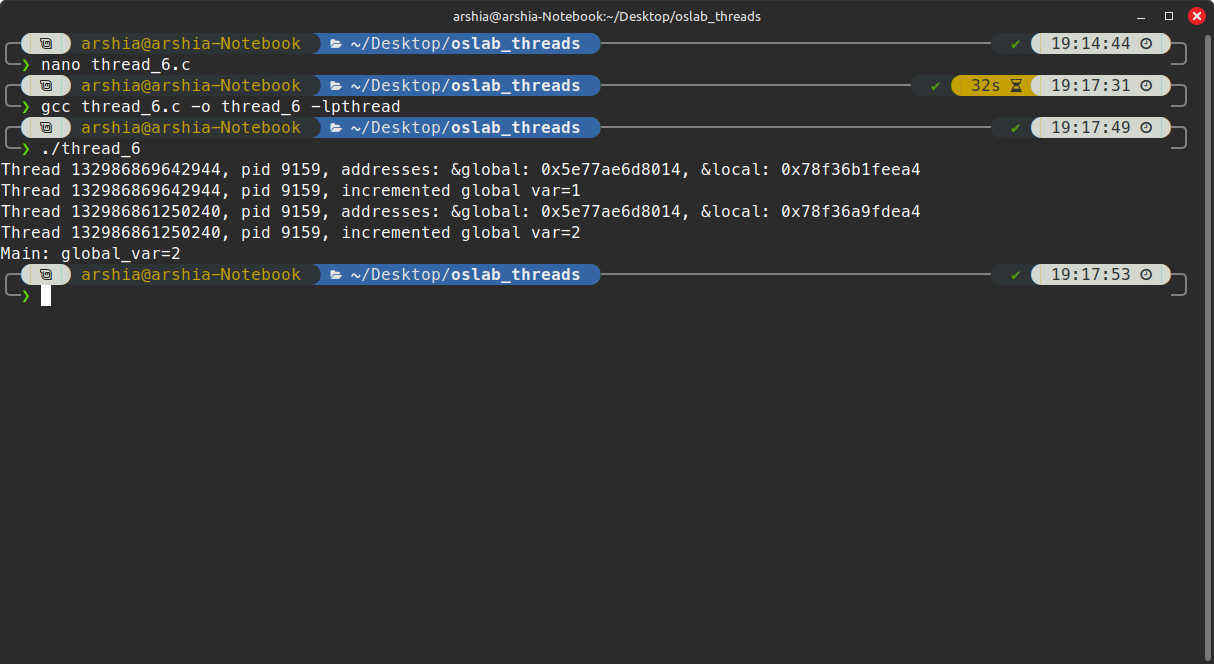
\includegraphics[width=\textwidth]{report7-resources/12.png}
		\caption{گام‌های کامپایل و اجرای برنامه شکل \ref{img:11}}
		\label{img:12}
	\end{figure}
	\subsection{}
	در این قسمت همان کار قسمت قبل را با پردازه‌ها انجام می‌دهیم. شکل \ref{img:13} برنامه و شکل \ref{img:14} اجرای آن را نشان می‌دهد.
	\begin{figure}[H]
		\centering
		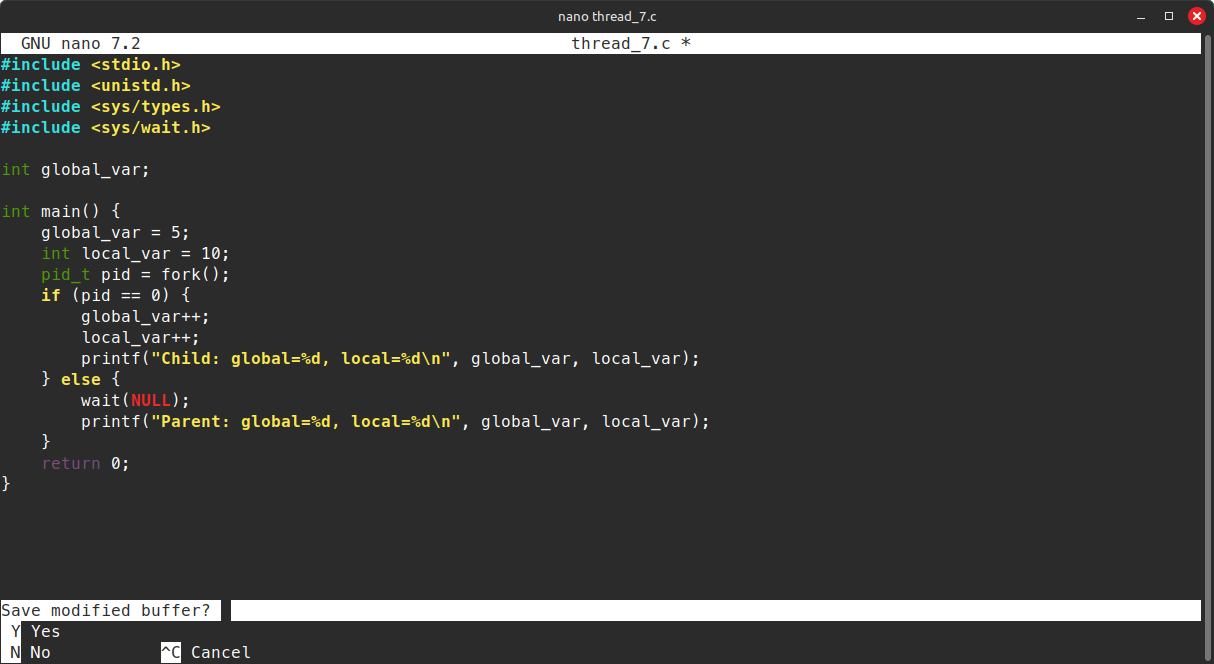
\includegraphics[width=\textwidth]{report7-resources/13.png}
		\caption{دسترسی به متغیر عمومی از پردازه والد و فرزند}
		\label{img:13}
	\end{figure}
	\begin{figure}[H]
		\centering
		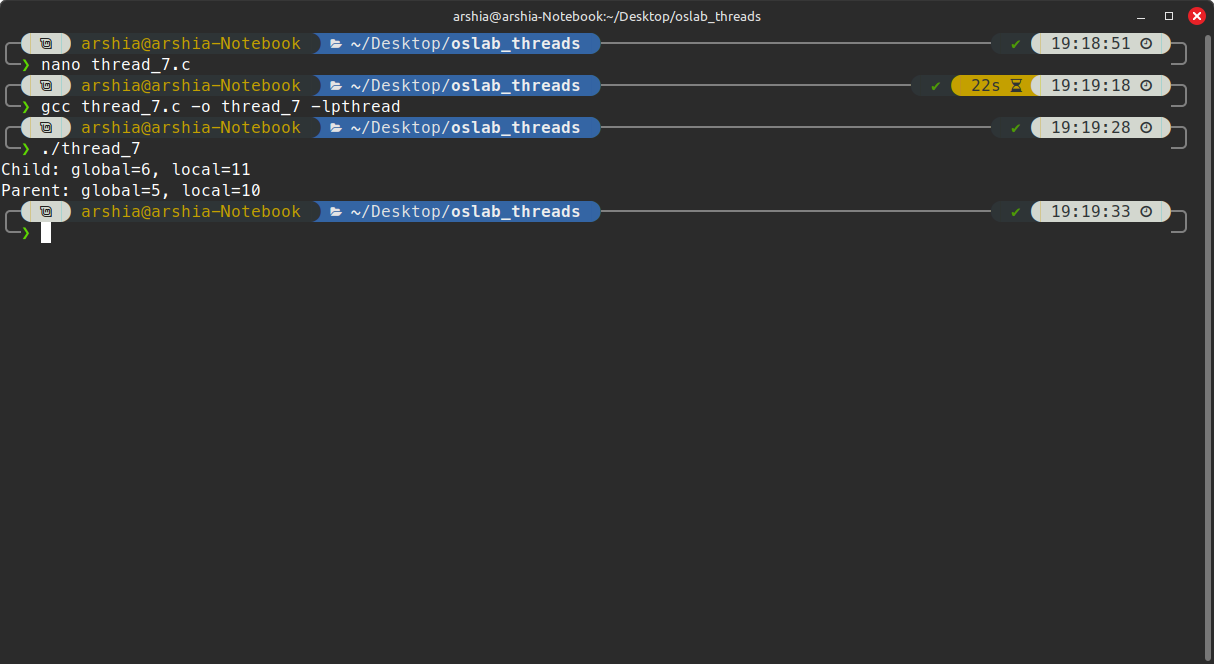
\includegraphics[width=\textwidth]{report7-resources/14.png}
		\caption{گام‌های کامپایل و اجرای برنامه شکل \ref{img:13}}
		\label{img:14}
	\end{figure}
	\newpage
	\section{پاس دادن متغیر به ریسه‌ها}
	در این قسمت پاس دادن ساختار‌ها به ریسه‌ها را بررسی می‌کنیم که محدودیت یک پارامتر ورودی به ریسه را حل می‌کند. شکل \ref{img:15} برنامه و شکل \ref{img:16} اجرا را نشان می‌دهد.
	\begin{figure}[H]
		\centering
		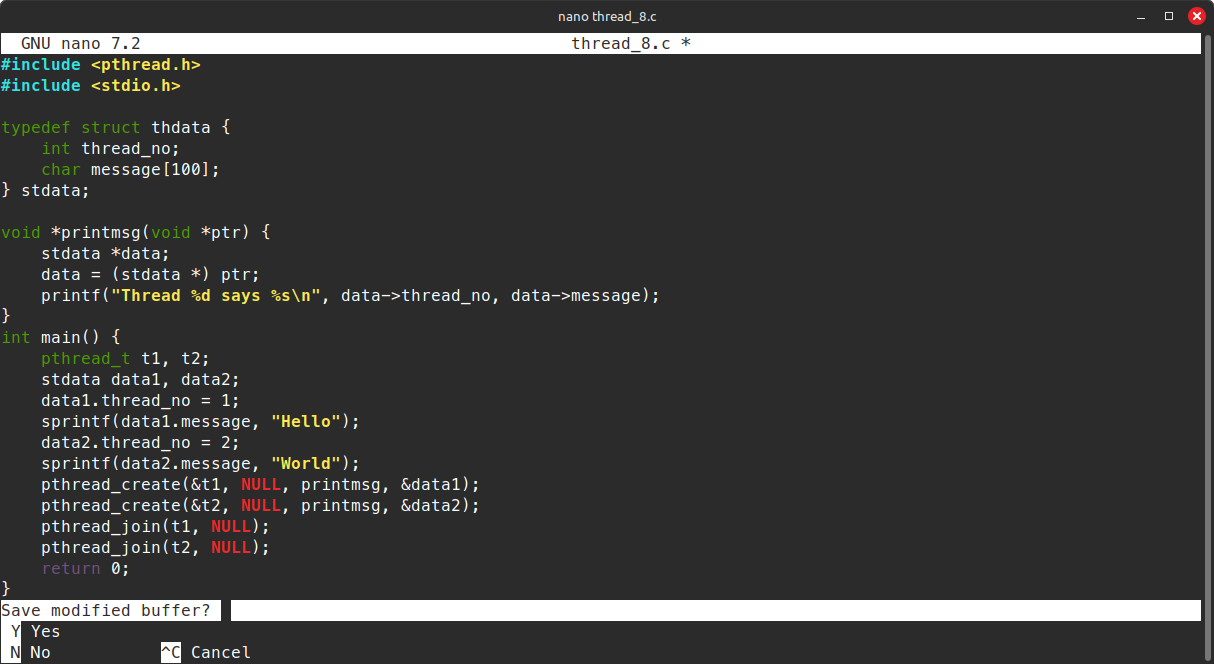
\includegraphics[width=\textwidth]{report7-resources/15.png}
		\caption{پاس دادن داده در غالب ساختار به ریسه و دسترسی به آن}
		\label{img:15}
	\end{figure}
	\begin{figure}[H]
		\centering
		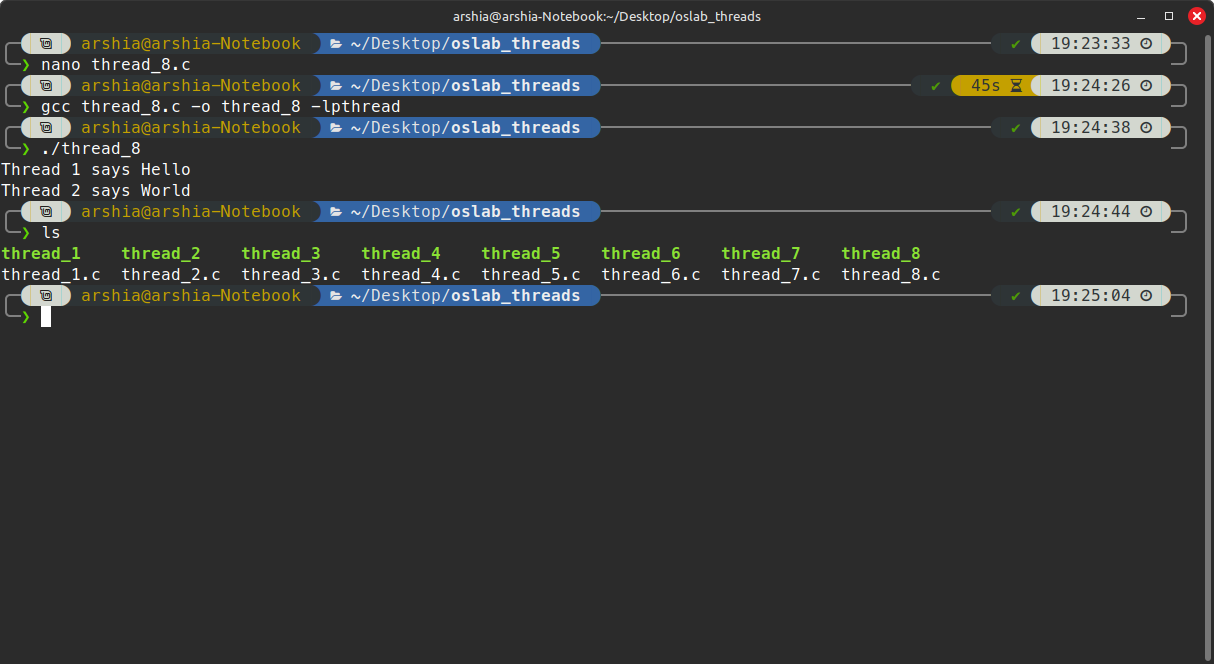
\includegraphics[width=\textwidth]{report7-resources/16.png}
		\caption{گام‌های کامپایل و اجرای برنامه شکل \ref{img:15}}
		\label{img:16}
	\end{figure}
        
	% ==============================
	% References
	% ==============================
	\newpage
	\begin{LTR}
		\printbibliography[title={مراجع}]
	\end{LTR}

	
\end{document}

